% 2010 年上海卷理科第 13 题：双曲线 x^2/4-y^2=1 的渐近线与直线 x=2 交于 E1、E2。
% 来源 PDF：普通高考/2010/2010上海理.pdf，SHA-256 e6181a8e02bfda976d5a2cee9432881769c184da4d3fca3b5a4d75c57a497ec6。
% 原页：第 1 页（A3 三栏）第 3 栏中部，书页码 627。
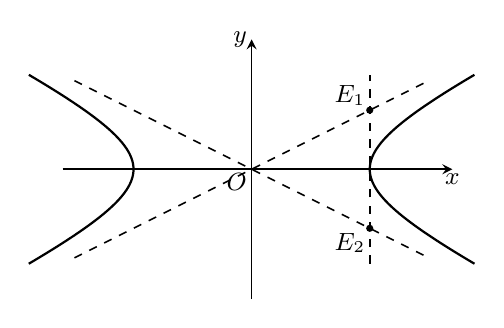
\begin{tikzpicture}[semithick, x=0.75cm, y=0.75cm, every node/.style={inner sep=1.4pt, font=\small}]
  \draw[-stealth] (-3.2,0) -- (3.4,0) node[below] {$x$};
  \draw[-stealth] (0,-2.2) -- (0,2.2) node[left] {$y$};
  \node[below left] at (0,0) {$O$};
  % 双曲线两支
  \draw[domain=-1.6:1.6,samples=80,thick] plot ({2*sqrt(1+\x*\x)},\x);
  \draw[domain=-1.6:1.6,samples=80,thick] plot ({-2*sqrt(1+\x*\x)},\x);
  % 渐近线
  \draw[dashed] (-3,-1.5) -- (3,1.5);
  \draw[dashed] (-3,1.5) -- (3,-1.5);
  % x=2
  \draw[dashed] (2,-1.6) -- (2,1.6);
  \fill (2,1) circle (1.3pt);
  \fill (2,-1) circle (1.3pt);
  \node[above left] at (2,1) {$E_1$};
  \node[below left] at (2,-1) {$E_2$};
\end{tikzpicture}
